\chapter{Exercícios}

\section{1º/2012}
\begin{exercicio}
  {1º/2012}{Arquiteturas de SO}
  {Admita um sistema operacional que é originalmente organizado segundo a estruturação microkernel no qual foi embutido um outro sistema operacional monolítico, por razões de desempenho. Como você classificaria esse sistema operacional? Por quê?}
\end{exercicio}

\begin{exercicio}
  {1º/2012}{Escalonamento de Processos}
  {Os escalonadores round-robin mantém, normalmente, uma fila de processos prontos, onde cada processo aparece uma só vez. Considere uma fila de prontos que mantém ponteiros para a tabela de processos. Qual seria o efeito de colocar dois ponteiros para o mesmo processo na fila de prontos $(A \rightarrow B \rightarrow C \rightarrow B)$?
  }

  O processo rodaria duas vezes por rodada, como se tivesse o dobro do quantum ou uma prioridade maior que os outros.
\end{exercicio}

\begin{exercicio}
  {1º/2012}{Escalonamento de Processos}
  {Considere o conjunto de $5$ processos e respectivos tempos de execução (quantum = $8$ms). \\
  A ordem de chegada dos processos foi $A \rightarrow B \rightarrow C \rightarrow D \rightarrow E$ (do mais antigo para o mais recente). No momento de início de execução do algoritmo de escalonamento, todos os processos estão prontos. Diga a ordem na qual este conjunto será executado, considerando as políticas \textit{Round-Robin} e \textit{Shortest Job First (SJF)}.
  \begin{table}[!h]
      \centering
      \begin{tabular}{cc}
        \hline \hline
        \textbf{Processo} & \textbf{Tempo de execução (ms)} \\ \hline
        A                 & 9                               \\
        B                 & 20                              \\
        C                 & 2                               \\
        D                 & 6                               \\
        E                 & 18                              \\
        \hline \hline
      \end{tabular}
      \caption{Tabela de Processos}
      \label{tab:ex3}
    \end{table}
  }

  Resposta aqui
\end{exercicio}

\begin{exercicio}
  {1º/2012}{Memória/Paginação}
  {Explique como funcionam as organizações, \textit{forward-mapped} (mapeamento direto) e tabela invertida, de páginas.}
\end{exercicio}

\begin{exercicio}
  {1º/2012}{Memória/Paginação}
  {Considere um sistema com espaço de endereçamento de $32$ bits e páginas de $4$KBytes e espaço de endereçamento real de $26$ bits.
  \begin{enumerate}[label=(\alph*)]
    \item Quantas entradas são necessárias em uma tabela de páginas forward-mapped?
    \item E na tabela de páginas invertida?
  \end{enumerate}}
\end{exercicio}

\begin{exercicio}
  {1º/2012}{Drivers}
  {O que é uma controladora? Qual entidade do SO interage com ela?}

\end{exercicio}

\begin{exercicio}
  {1º/2012}{Sistemas de Arquivo}
  {Alguns sistemas de arquivo deletam todos os arquivos de usuário quando o usuário se desconecta da máquina (\textit{logoff}), a não ser que o usuário, explicitamente, diga quais arquivos devem ser permanentes. Comente esta abordagem em relação à abordagem tradicional.}
\end{exercicio}

\begin{exercicio}
  {1º/2012}{Sistemas de Arquivo}
  {Sobre \textit{buffer cache}:
  \begin{enumerate}[label=(\alph*)]
    \item Explique como as leituras e escritas em arquivos convencionais funcionam quando existe buffer cache.
    \item Explique como as leituras e escritas em arquivos convencionais funcionam quando não existe buffer cache.
  \end{enumerate}}
\end{exercicio}

\begin{exercicio}
  {1º/2012}{Processos (Deadlock)}
  {Apresente uma solução para o problema do produtor-consumidor utilizando unicamente locks.}
\end{exercicio}

\begin{exercicio}
  {1º/2012}{Processos/Escalonamento}
  {O algoritmo de escalonamento de processos FCFS pode ser considerado um caso particular do algortimo Round-Robin. Qual é esse caso?}
  Quando o quantum é infinito (teoricamente), na prática utiliza-se como FFFF ($32$ bits) FFFF FFFF( $64$ bits).
\end{exercicio}

\begin{exercicio}
  {1º/2012}{Memória/Paginação}
  {Considere a seguinte sequência de referências à páginas:
  1,2,3,4,2,1,5,6,2,1,2,3,7,6,3,2,1,2,3,6 \\
  Quantos page faults ocorrerão para os algoritmos FCFS, ótimo e LRU, supondo que a memória real possui $4$ frames? Considere que inicialmente a memória está vazia.}
\end{exercicio}

\begin{exercicio}
  {1º/2012}{Virtualização}
  {Os conceitos de \textit{full virtualization} e para \textit{virtualization} são explicados abaixo:\\
  \textit{Full Virtualization} oferece uma abstração de máquina virtual que é uma cópia exata do hardware e, portanto, permite hospedar sistemas operacionais inalterados.\\
  \textit{Virtualization} oferece uma abstração de máquina virtual que é similar, porém, não idêntica ao hardware e, por isso, requer que algumas modificações sejam feitas no sistema operacional hospedado.
  Sabendo disso, qual estrutura de sistema operacional suporta \textit{full virtualization} e qual suporta para \textit{virtualization}? Justifique sua resposta.}
\end{exercicio}

\begin{exercicio}
  {1º/2012}{Organização de Sistemas Operacionais}
  {Complete o quadro abaixo com os valores (A - Alto, M - Médio, B - Baixo). Justifque sua resposta. Atenção: Cada linha deve conter os valores Alto, Médio e Baixo.
  \begin{table}[!h]
    \centering
    \caption{Tabela de comparação entre organizações}
    \label{tab:ex15}
    \begin{tabular}{clll}
      \hline \hline
    \multicolumn{1}{l}{}             & \multicolumn{1}{c}{\textbf{Monolítico}} & \multicolumn{1}{c}{\textbf{MicroKernel}} & \multicolumn{1}{c}{\textbf{ExoKernel}} \\ \hline
    \textbf{Flexibilidade}           &                                         &                                          &                                        \\
    \textbf{Visão Global do Sistema} &                                         &                                          &                                        \\ \hline \hline
    \end{tabular}
    \end{table}}
\end{exercicio}





\section{1º/2013}
\begin{exercicio}
  {1º/2013}{Sistemas de Arquivo}
  {Considere um arquivo de alocação contígua composto por 100 blocos, cujo tamanho máximo é 200 blocos. Quantas operações devem ser feitas caso:
  \begin{enumerate}
    \item Um bloco seja adicionado no início do arquivo.
    \item Um bloco seja adicionado no final do arquivo.
    \item Um bloco seja removido no início do arquivo.
  \end{enumerate}
  Responda o mesmo para um arquivo de mesmo tamanho que utilize lista encadeada.}
\end{exercicio}

\begin{exercicio}
  {1º/2013}{\textit{Esclonamento de processos}}
  {Considere o conjunto de $5$ processos e respectivos tempos de execução (quantum=$8$ms).
  A ordem de chegada dos processos foi $A \rightarrow B \rightarrow C \rightarrow D \rightarrow E$ (do mais antigo para o mais recente). No momento de início de execução do algoritmo de escalonamento, todos os processos estão prontos. Diga a ordem na qual este conjunto será executado, considerando as políticas \textit{Round-Robin} e \textit{Shortest Job First (SJF)}.

  \begin{table}[!h]
    \centering
    \caption{Tabela de Processos}
    \label{tab:ex3}
    \begin{tabular}{cc}
    \hline \hline
    \textbf{Processo} & \textbf{Tempo de execução (ms)} \\ \hline
    A                 & 9                               \\
    B                 & 2                              \\
    C                 & 7                               \\
    D                 & 1                               \\
    E                 & 18                              \\ \hline \hline
    \end{tabular}
    \end{table}}
\end{exercicio}

\begin{exercicio}
  {1º/2013}{Processos (Threads)}
  {Explique os $2$ níveis de implementação de threads. Cite vantagens e desvantagens.}
\end{exercicio}





\section{1º/2017}
\begin{exercicio}
  {2º/2017}{\textit{Threads}}
  {Por quê a implementação de \textit{threads} em nível de usuário possui um custo extremamente baixo de troca de contexto?}

  Pois não possui o custo da troca de modo usuário para modo protegido.
\end{exercicio}

\begin{exercicio}
  {2º/2017}{Condições de Corrida}
  {Considere o código multi-processo abaixo. Existe condição de corrida nesse código? Se sim, corrija o código de maneira a eliminá-la.}
\end{exercicio}

\begin{exercicio}
  {2º/2017}{\textit{Deadlocks}}
  {Por quê \textit{deadlocks} são ditos \textit{stable properties}?}

  Pois consistem em estados que não podem ser mudados sem utilização de força externa.
\end{exercicio}

\begin{exercicio}
  {2º/2017}{Arquivos}
  {Qual a função da operação \texttt{OPEN} e \texttt{CLOSE}?}

  \texttt{OPEN:} fazer a associação entre o processo e o arquivo, através da tabela de descritores, retornando um descritor que será usado nas próximas operações.

  \texttt{CLOSE}: desfazer a associação entre processo e arquivo, tornando o descritor indisponível.
\end{exercicio}

\begin{exercicio}
  {2º/2017}{Memória Virtual}
  {
    Considere um sistema de memória virtual paginada. Dê os nomes dos elementos marcados com (a), (b), (c) e (d) na figura abaixo e explique como cada um é utilizado em uma operação de acesso à memória.
    \begin{figure}
      \centering
      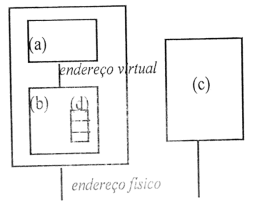
\includegraphics[width=0.4\textwidth]{ex-mem-structure}
    \end{figure}
  }

  \begin{enumerate}[label=(\alph*)]
    \item \textbf{CPU:} envia o endereço virtual à MMU;

    \item \textbf{MMU:} quebra o endereço virtual em duas partes, sendo elas a página e o deslocamento. A MMU usa $p$ como índice na TLB para obter o \textit{frame} $f$. A MMU troca a página $p$ pelo frame $f$, que é jogado no barramento junto com o deslocamento.

    \item \textbf{Memória RAM:} entidade que guarda o dado desejado e será acessada;

    \item \textbf{Tabela de Páginas:} guarda % TODO: completar
  \end{enumerate}
\end{exercicio}


\begin{exercicio}
  {2º/2017}{Paginação}
  {Considere um sistema com 4 \textit{frames} e 8 páginas. Admita a seguinte \textit{string} de referência: 0172327103. Quantos \textit{page faults} ocorrerão se o algorítmo de substituição for FIFO? E se for LRU?}

  Fazer o exercício de forma a mostrar cada iteração e o histórico das tabelas.

  FIFO: 6 page faults

  LRU: 7 page faults
\end{exercicio}

\begin{exercicio}
  {2º/2017}{Estruturação de Sistemas Operacionais}
  {Explique a estruturação em camadas de sistema operacional. Comente vantagens e desvantagens.}

\end{exercicio}

\begin{exercicio}
  {2º/2017}{Arquiteturas de SO/Processos}
  {Cite os passos para a criação de processos nas arquiteturas monolíticas, \textit{microkernel} e \textit{exokernel}.}

  Para as \textsc{arquiteturas monolíticas}:
  \begin{enumerate}
    \item O processo pai solicita a criação de um processo filho, através de uma \textit{chamada de sistema} \texttt{create process};

    \item O SO aloca uma entrada livre na \textit{tabela de processos} para o processo filho;

    \item O SO atribui um \textit{PID} ao processo filho;

    \item O SO ajusta a \textit{área de memória} para a execução do processo filho;
    \begin{itemize}
      \item % TODO: o que faz quando é criação tradicional?
      \item % TODO: o que faz quando é clonagem?
    \end{itemize}

    \item O SO preenche os \textit{valores de registradores} para execução do processo filho na tabela de processos;

    \item O SO insere o processo filho na fila \textit{ready} do escalonador;

    \item O SO retorna ao processo pai.
  \end{enumerate}

  Para o \textsc{microkernel}:
  \begin{enumerate}
    \item O processo pai envia uma mensagem para o microkernel, colocando o \texttt{create process} como conteúdo;

    \item O microkernel recebe a mensagem e determina que o processo filho deve ser criado;

    \item O microkernel aloca uma entrada livre na \textit{tabela de processos} para o processo filho;

    \item O microkernel atribui um \textit{PID} ao processo filho;

    \item O microkernel ajusta a \textit{área de memória} para a execução do processo filho;

    \item O microkernel preenche os \textit{valores de registradores} para execução do processo filho na tabela de processos;

    \item O microkernel insere o processo filho na fila \textit{ready} do escalonador;

    \item O microkernel envia uma mensagem para o processo pai contendo o valor de retorno.
  \end{enumerate}

  Para o \textsc{exokernel}:
  \begin{enumerate}
    \item O processo pai solicita a criação de um processo filho para a LibOS, através de uma \textit{chamada de função} \texttt{create process};

    \item A LibOS aloca uma entrada livre na \textit{tabela de processos} para o processo filho;

    \item A LibOS atribui um \textit{PID} ao processo filho;

    \item A LibOS pede uma região de software (área de memória) ao exokernel, via \textit{chamada de sistema}. Esta área é destinada ao processo filho;

    \item A LibOS solicita um \textit{processor environment} (PE), via chamada de sistema, e copiar o valor dos registradores para lá;

    \item A LibOS preenche o de prólogo e epílogo do PE (troca de contexto), descarregando o código;

    \item O exokernel coloca o PE na sua fila \textit{ready};

    \item A LibOS coloca o processo na sua fila \textit{ready};

    \item A LibOS retorna ao processo pai.
  \end{enumerate}

\end{exercicio}
